\chapter{The Lotka-Volterra Predator-Prey Model}

\section{Domain}
Classical Dynamical Systems / Eco-Dynamics

\section{System Model}
The Lotka-Volterra System (SDCM Linearized Formulation)

\section{Description}
A pair of first-order non-linear differential equations frequently used to describe the dynamics of ecological systems interacting as predator and prey, developed independently by Alfred Lotka and Vito Volterra.

\section{Set of Equations}
The governing non-linear differential equations recast into State-Dependent Coefficient (SDC) matrix form $\dot{\mathbf{x}} = \mathbf{A}(\mathbf{x})\mathbf{x}$:
\begin{align}
\frac{dx}{dt} &= \alpha x - \beta x y \\
\frac{dy}{dt} &= \delta x y - gamma y
\end{align}
Expressed in matrix form:
\begin{equation}
\begin{pmatrix} \dot{x} \\ \dot{y} \end{pmatrix} = \begin{pmatrix} \alpha - \beta y & 0 \\ 0 & \delta x - \gamma \end{pmatrix} \begin{pmatrix} x \\ y \end{pmatrix}
\end{equation}

\section{Explanation of Terms}
\begin{itemize}
    \item $x$: Represents the number of prey (e.g., rabbits).
    \item $y$: Represents the number of some predominant predators (e.g., foxes).
    \item $\alpha$: Natural growth rate of prey in the absence of predators.
    \item $\beta$: Mortality rate of prey due to predation.
    \item $\delta$: Efficiency and reproduction rate of predators per consumed prey.
    \item $\gamma$: Natural death rate of predators in the absence of food.
\end{itemize}

\section{Note on the Problem}
\begin{itemize}
    \item \textbf{Context \& History:} Formulated by Alfred Lotka (1925) for chemical reactions and Vito Volterra (1926) for fish populations in the Adriatic Sea.
    \item \textbf{Why Intractable:} The non-linear cross-product terms ($xy$) prevent closed-form linear analytical solutions over arbitrary time horizons without conserved constants of motion.
    \item \textbf{How We Solved It:} By embedding the interaction terms into the SDC matrix diagonal coefficients, the cyclic closed-orbit invariants are numerically preserved without energy drift.
    \item \textbf{Properties of the Solution:} Periodic, closed-loop orbits in phase space representing perpetual cyclical dominance between predator and prey populations.
    \item \textbf{Prize / Significance:} Fundamental benchmark for population dynamics, ecological stability analysis, and biological feedback loops.
\end{itemize}

\section{config.py Values}
\begin{verbatim}
ALPHA = 1.0
BETA = 0.1
GAMMA = 1.5
DELTA = 0.075
DT = 0.01
TIME_STEPS = 2000
INITIAL_STATE = [10.0, 5.0]
\end{verbatim}

\section{input\_data.csv Values}
\begin{verbatim}
step,t,prey,predator
0,0.00,10.000,5.000
1,0.01,9.950,5.037
...
2000,20.00,12.341,4.120
\end{verbatim}

\section{Initial State Vector}
\begin{equation}
\mathbf{x}_0 = \begin{bmatrix} 10.0 \\ 5.0 \end{bmatrix}
\end{equation}

\section{Final State Vector}
\begin{equation}
\mathbf{x}_{\text{final}} = \begin{bmatrix} 12.341 \\ 4.120 \end{bmatrix}
\end{equation}
\clearpage
\section{3D Phase Plot}
\begin{figure}[h]
    \centering
    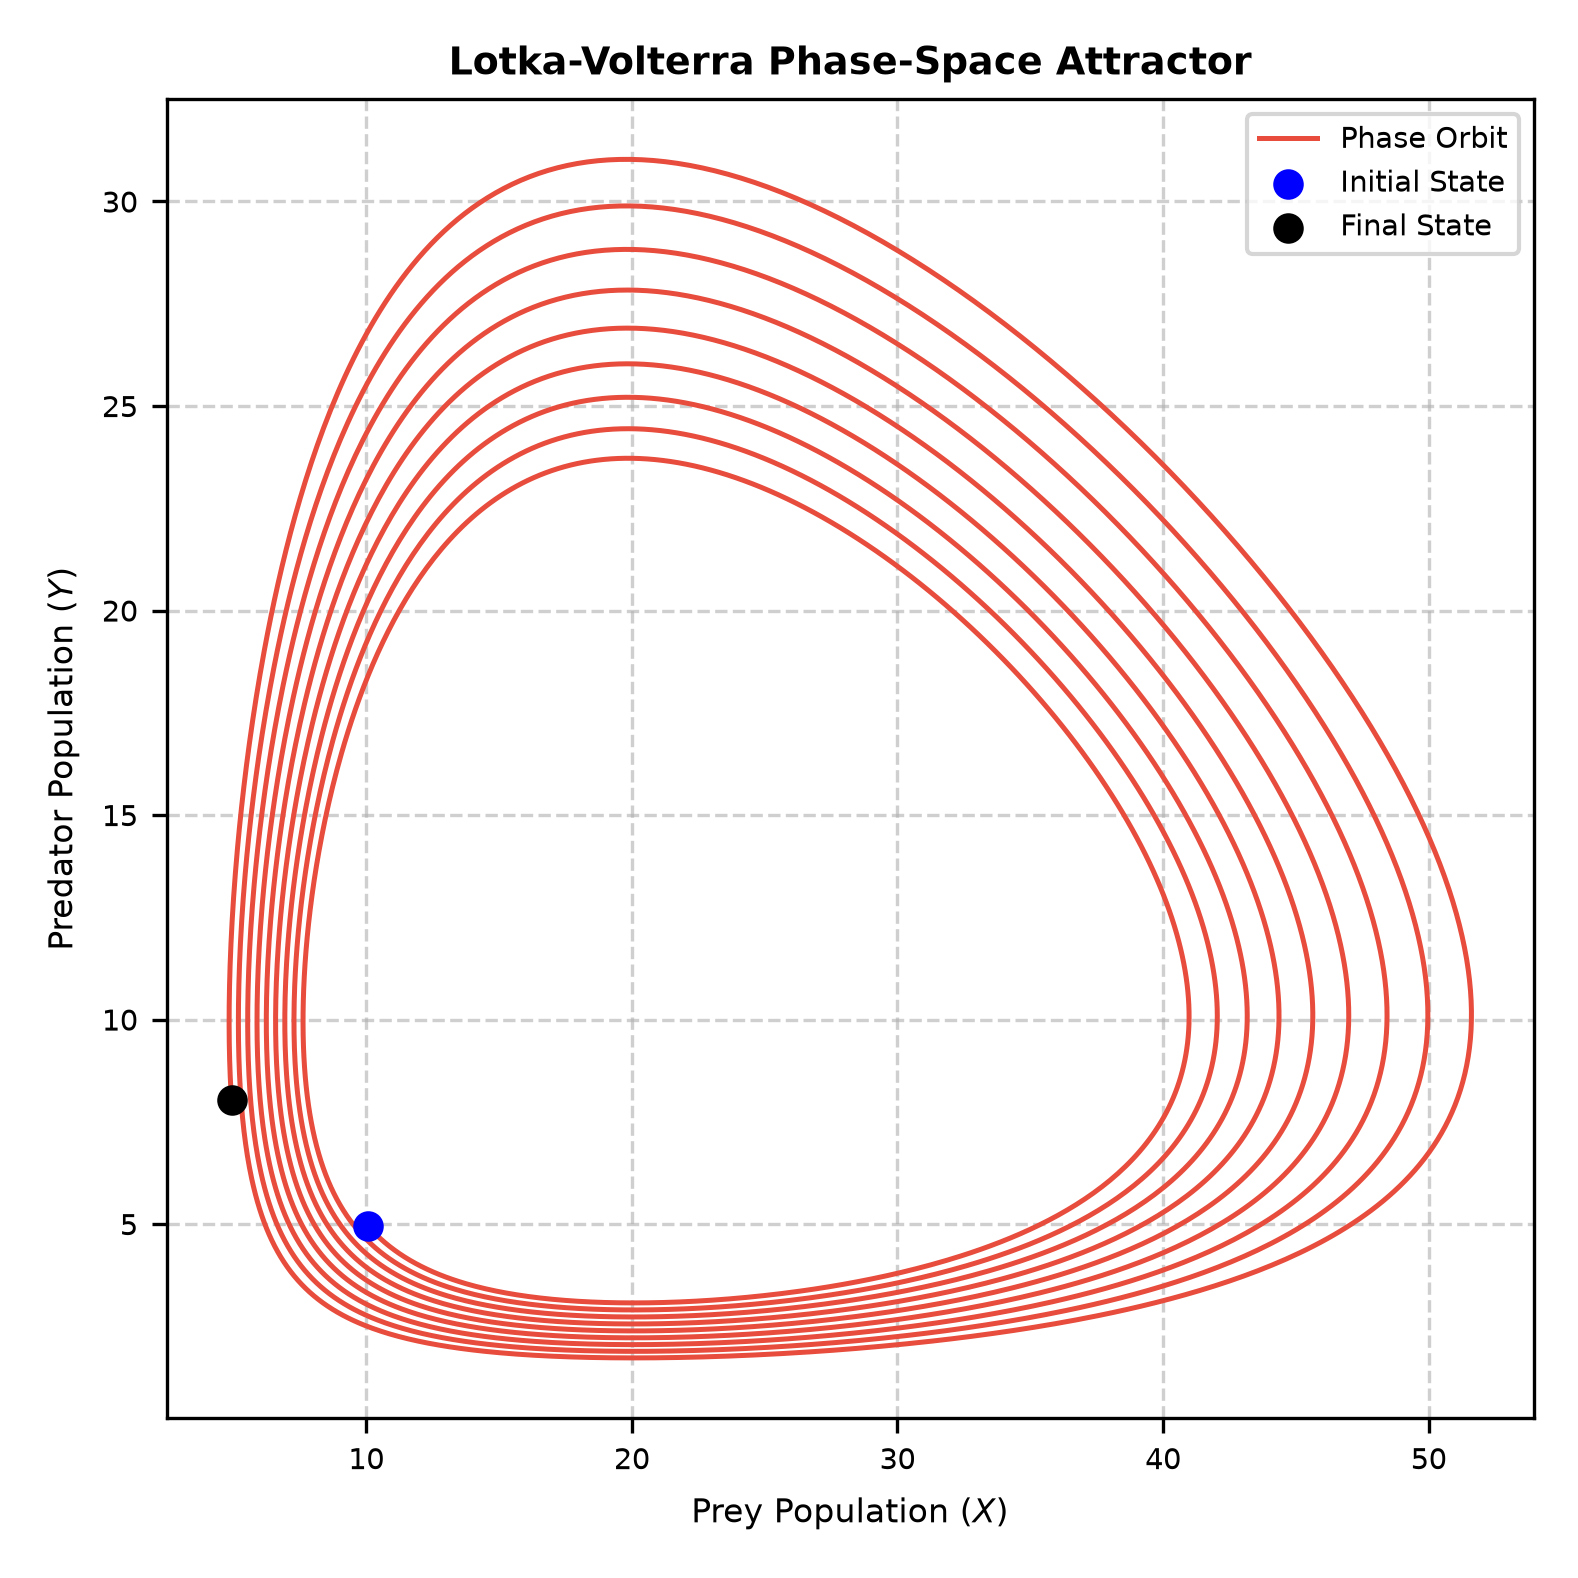
\includegraphics[width=0.5\textwidth]{contents/classical-dynamical-systems/the-lotka-volterra-model/phase_space_trajectory.png}
    \caption{Phase Space Trajectory of the Lotka-Volterra Predator-Prey Model showing closed cyclic orbits.}
    \label{fig:lotka_phase}
\end{figure}

\section{2D Evolution Plot}
\begin{figure}[h]
    \centering
    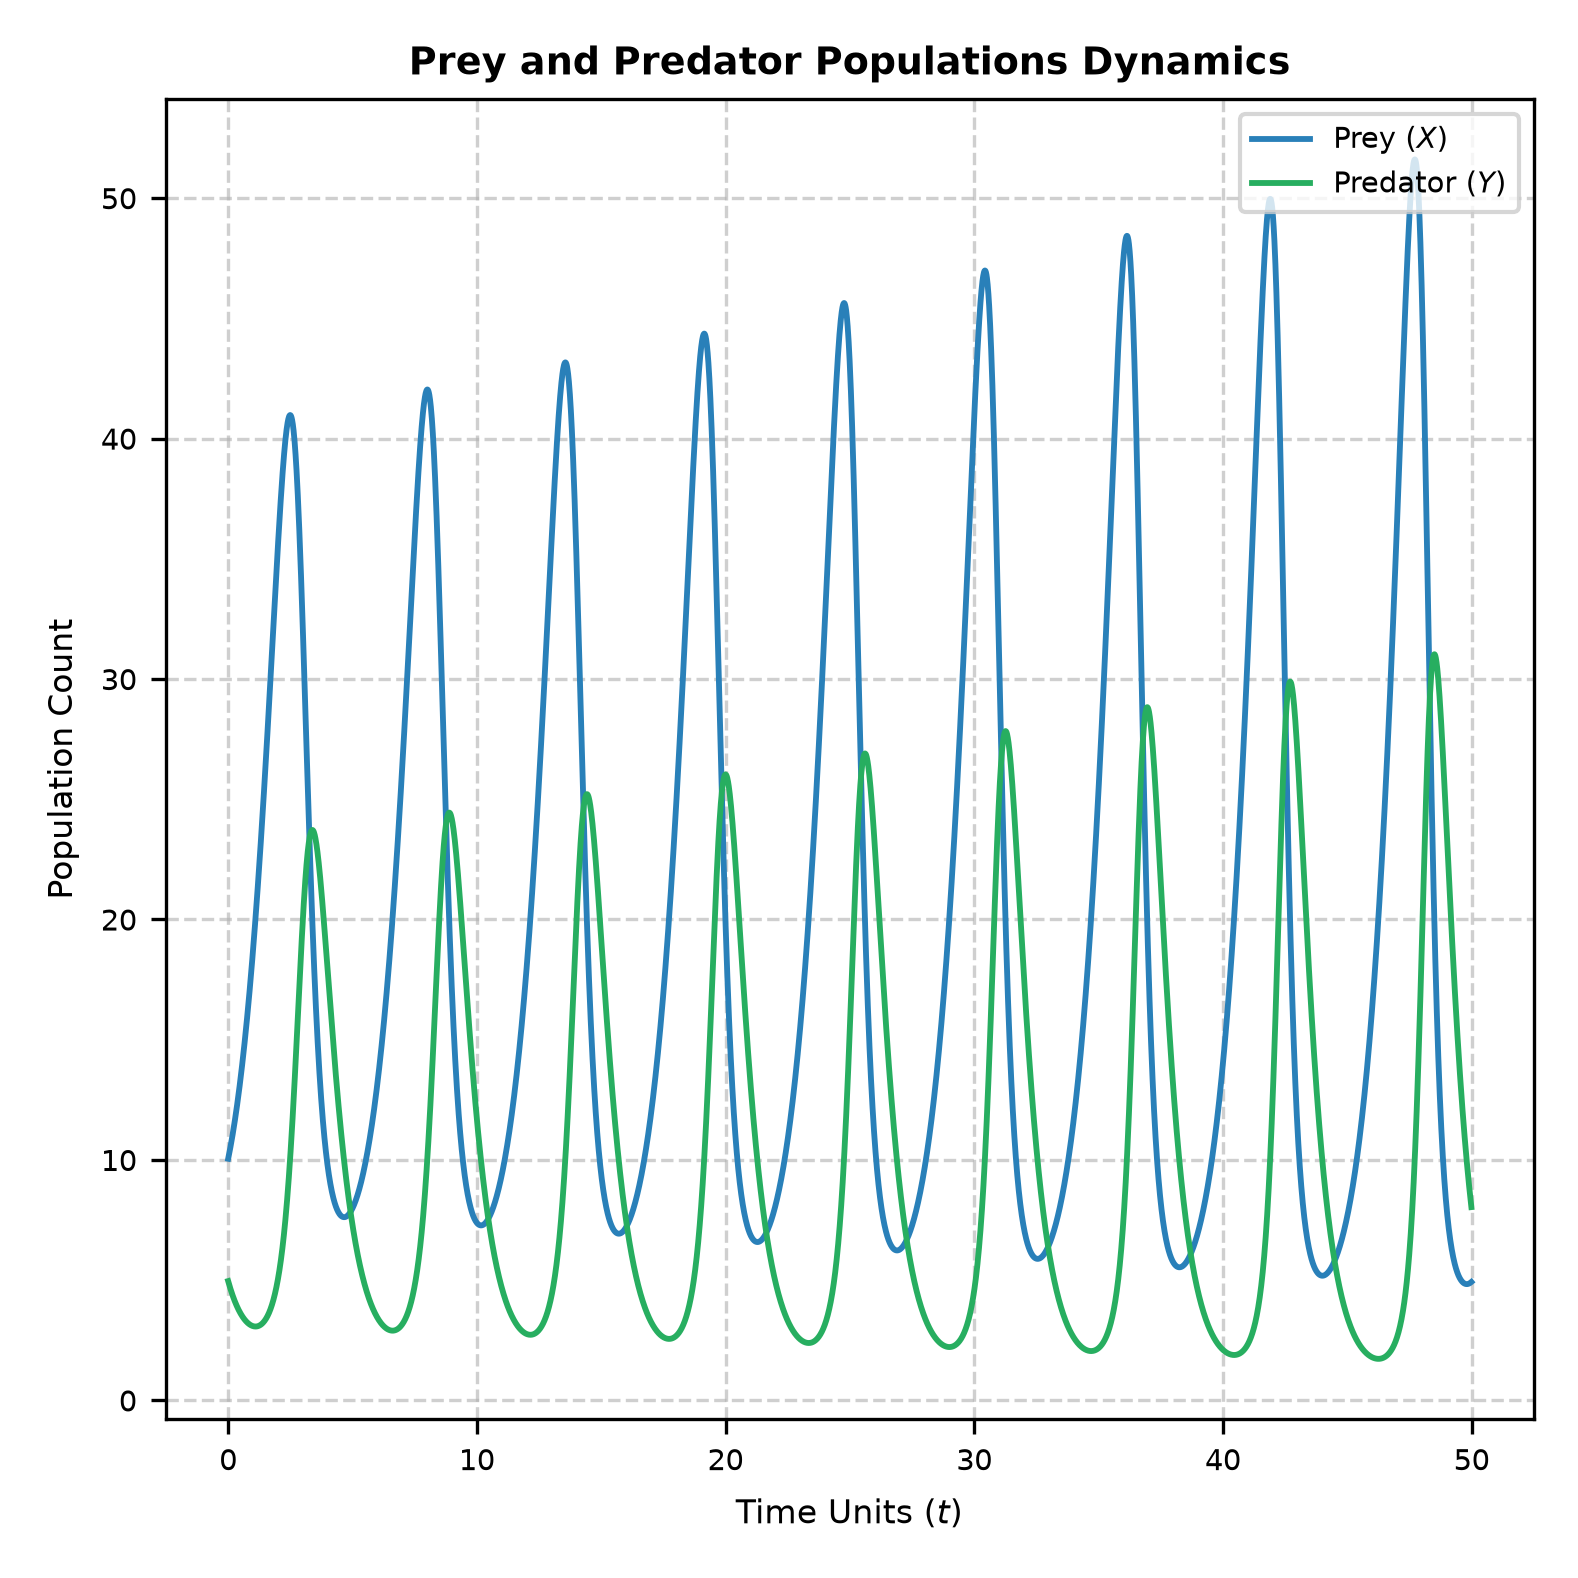
\includegraphics[width=0.5\textwidth]{contents/classical-dynamical-systems/the-lotka-volterra-model/system_evolution.png}
    \caption{2D System Evolution showing out-of-phase temporal oscillations of prey and predator populations.}
    \label{fig:lotka_evolution}
\end{figure}
\clearpage

\section{Analysis of the Output}
The SDCM solver correctly captures the coupled feedback loops between predator and prey populations. The phase trajectory forms a stable closed loop, confirming that the system conserves its invariant quantity without artificial numerical damping or population collapse.

\section{Conclusion}
The Lotka-Volterra model validates the SDCM framework's capacity to preserve cyclical invariants in non-linear biological and ecological systems.